\documentclass[11pt]{article}

\usepackage{booktabs}
\usepackage{dcolumn} 
\usepackage{epstopdf}
\usepackage{fourier}
\usepackage{fullpage}
\usepackage{graphicx}
\usepackage{hyperref}
\usepackage{longtable} 
\usepackage{natbib}
\usepackage{rotating}
\usepackage{tabularx}
\usepackage{amsmath}
% \usepackage{algorithmic} 
% \usepackage{algorithm2e}

\hypersetup{
  colorlinks = TRUE,
  citecolor=blue,
  linkcolor=red,
  urlcolor=black
}

\begin{document} 

\title{Perceived Wages}

\date{\today}

\author{ John J. Horton \\ NYU Stern\footnote{Author contact information, datasets and code are currently or will be available at \href{http://www.john-joseph-horton.com/}{http://www.john-joseph-horton.com/}. } }
\maketitle

\begin{abstract}
\noindent  Using a convenience sample of workers, I test their perceptions of hourly wages and actual hourly wages for the top one hundred BLS occupations, as measured by employment. 
Estmation errors are decreasing in the prevelance of an occupation. 
Knowing someone who has that occupation also decreases error rates. 
There appears to be a U-shaped pattern in knowledge about occupations
Workers do not appear to know random subsets of people with an occupation: knowledge is substantially clustered. \newline 
\newline 
\noindent JEL J01, J24, J3
\end{abstract} 

\section{Introduction}

Workers need know what various occupations pay--and will pay in the future---to plan their careers. 
Systematic informational gaps could be consequential, leading to misallocation of job search efforts and human capital investments. 
However, to the extent that these gaps exist, they might be cheaply fixable: 
several studies have highlighted the powerful effects obtainable from purely informational interventions (e.g., \cite{jensen2010perceived}, \cite{dupas2009teenagers}, \cite{card2010inequality}). 
At least part of the motivation of government statistical efforts like the OES is precisely this allocative efficiency goal. 

The purpose of this study is to measure information gaps and explore whether any patterns emerge across occupations. 
This was done using a convenience sample of US-based workers on their knowledge about the top (by May 2013 employment figures) 100 BLS occupations.  
For each occupation, participants were asked: 
\begin{enumerate}
\item Whether they know what the job consists of 
\item Whether they know anyone with that job 
\item The hourly wage for that job 
\item Whether wages and employment for that occupation will rise or fall in the future.  
\end{enumerate} 

For each occupation, 30 evaluations were performed. 
The short time taken to answer questions suggests that workers are not doing research. 
There was no incentive for correct answers. 

The focus on the analysis was to:
-characterize performance and see whether the ``wisdom of crowds'' hypotheses holds.
-find poorly labeled occupations in the BLS/OES 
-see what occupations are misperceived. 
-see how total employment and social knowledge mediate performance in estimating hourly wages 
-test whether social knowledge is ``segmented'' by wage  

There is substantial variation across occupations in whether they are known by the sample. 
First, individual error rates (MSE between predicted and actual hourly wage) are decreasing the total employment in that occupation. 
This is both re-assuring and unsurprising. 
Suggesting a mechanism, the more people workers know with that occupation, the better their estimates.  
Knowledge of an occupation seems to be substantially wage-biased, in that workers are more accurate when predicting the hourly wage of low-wage jobs. 
This is true in percentages.  
The wisdom of crowds hypotheses suggests that combining the noisy signals of a large number of individuals can lead to very accurate predictions. 
This is more or less the case here: the mean worker rating for each occupation explains 70\% of the variation in actual log hourly wages.  

%% This was the justification for including the Knowledge of the World of Work (KWW) test in the NLSY. 
%% The original KWW consisted of matching job descriptions to job titles and a section of relative comparisons of wages. 
%% The KWW was predictive of positive future economic success and was correlated with higher wages, greater tenure etc \citep{kohen1975133}. 
%% It is unclear whether KWW was just measuring intelligence of ability---KWW is sometimes used as an instrument for IQ to deal with measurement error. 

%\cite{snowberg2011prediction}
%\cite{kohen1975} 

\section{Results}

The sample of workers answering questions on MTurk. 
What we lack in representativeness, we gain in numbers. 

If a pattern or causal effect exists in one population, there is always a question of generalizability. 

\subsection{Discussion} 
What if the sample of respondents is just a sample of low-wage workers? 

- We can ask workers for their incomes 
- We can show in the literature that this is not a particularly biased group 
- We can use Google Survey, a nationally representative sample, to adjust 

What if high-way jobs are just less common?
Controlling for the total employment in that category does not make the effect go away. 

What if the hourly/annual salary throws things off? 

Do high-way jobs just have more variance? 

\subsection{Knowledge of what different occupations are} 

In Figure~\ref{fig:knoweldge_by_occupation}, we plot the mean knowledge index by occupations.  

\begin{figure}
\caption{Self-reported knowledge by BLS occupation title \label{fig:knowledge_by_occupation}} 
\centering
\begin{minipage}{0.95 \linewidth}
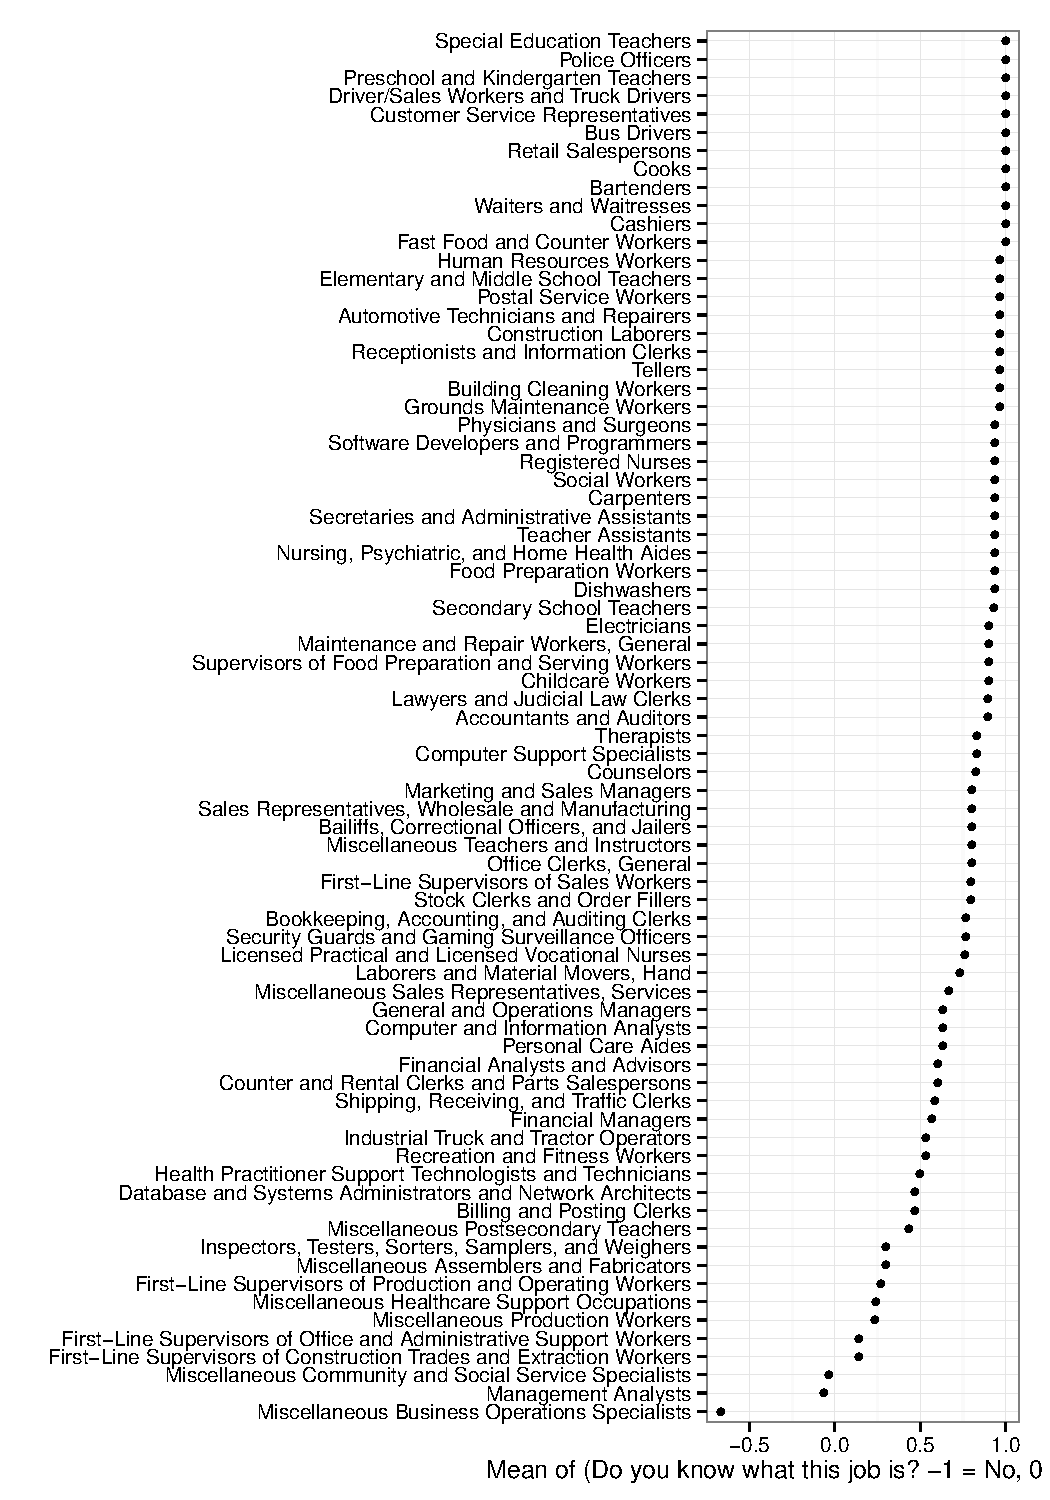
\includegraphics[width = \linewidth]{./plots/knowledge_by_occupation.pdf}
\end{minipage}  
\end{figure} 

In Figure~\ref{fig:knowledge_by_wage} we show the fraction of respondents reporting that they know what an occupation is, binned by hourly wage. 
A clear U-shaped pattern is apparent: respondnents know more about low- and high-wage occupations, but less about the middle. 
This probably reflects universal experience with low-wage jobs like waitressing and cleaning and high-wage professional jobs like doctor and lawyer. 

\begin{figure}
\caption{Hourly wage and occupational knowledge \label{fig:knowledge_by_wage}} 
\centering
\begin{minipage}{0.95 \linewidth}
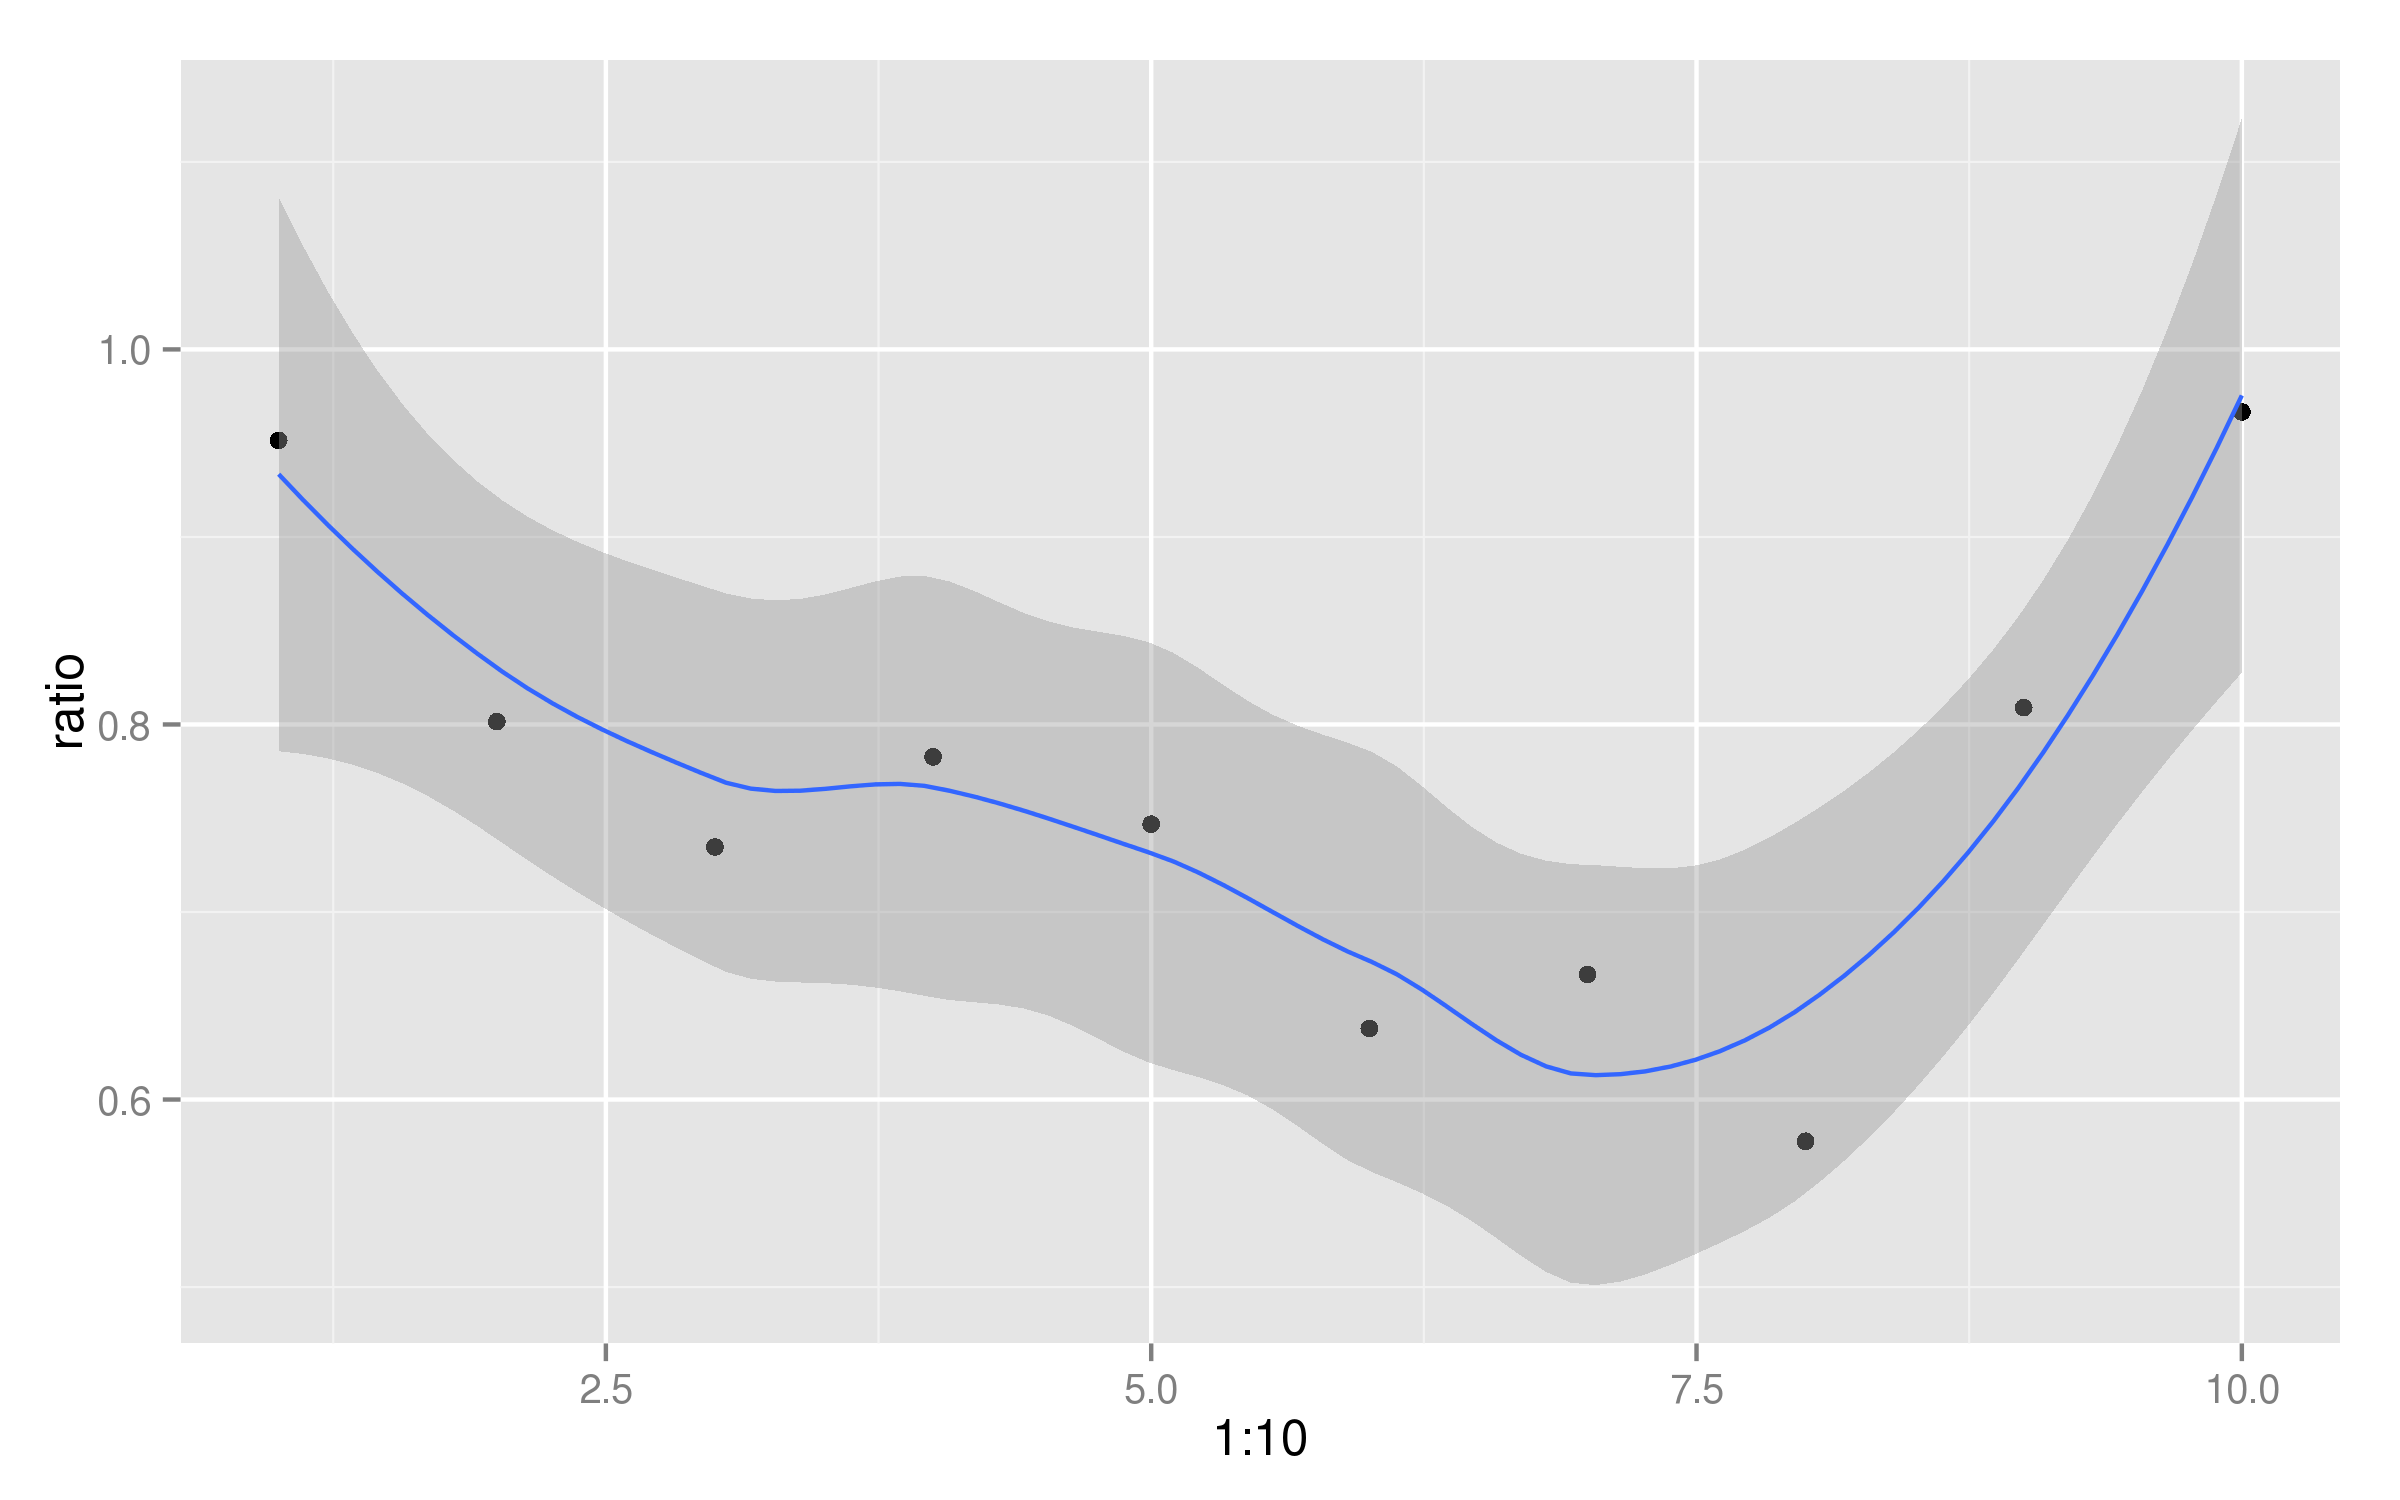
\includegraphics[width = \linewidth]{./plots/knowledge_wage.png}
\end{minipage}  
\end{figure} 

\subsection{Personal knowledge of someone working with an occupation} 

\begin{figure}
\caption{Social index by BLS occupation title} \label{fig:social_by_occupation}  
\centering
\begin{minipage}{0.95 \linewidth}
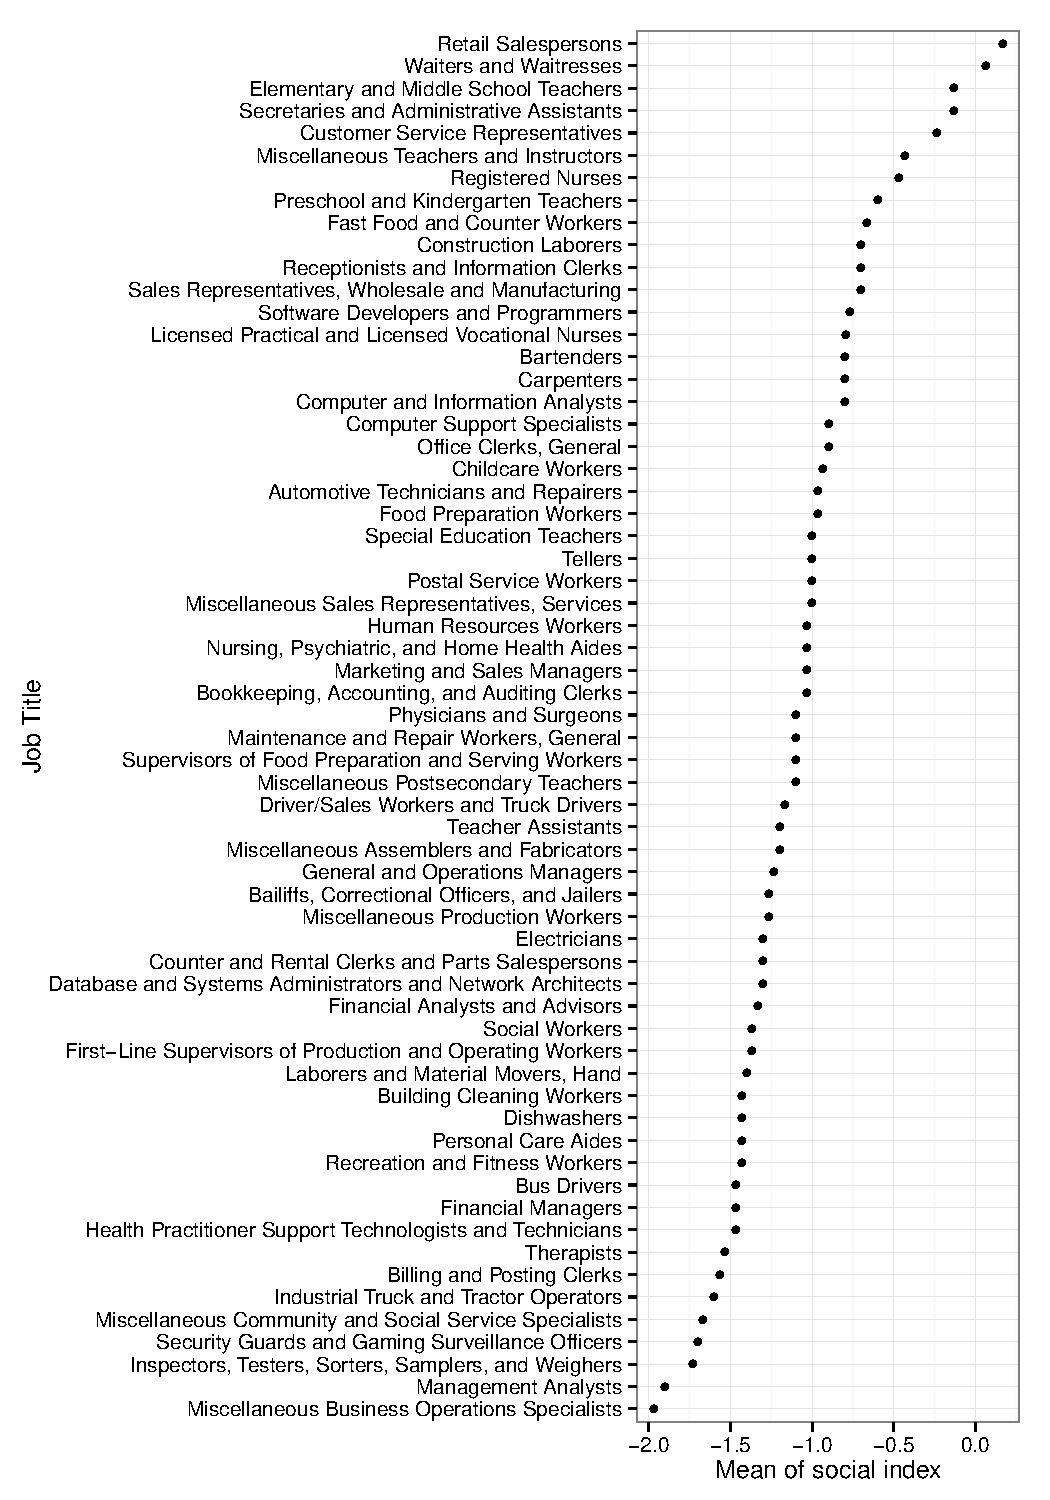
\includegraphics[width = \linewidth]{./plots/social_by_occupation.pdf}
\end{minipage}  
\end{figure} 

\subsection{Prediction} 

In Table~\ref{tab:error_prediction} we regress MSE in hourly wage estimates on a number of predictors. 

\begin{table}
\centering 
\caption{Mean square error of hourly wage predictions \label{tab:error_prediction}}

% Table created by stargazer v.4.5.3 by Marek Hlavac, Harvard University. E-mail: hlavac at fas.harvard.edu
% Date and time: Sat, Dec 14, 2013 - 07:27:59 AM
\begin{table}[!htbp] \centering 
  \caption{Fixed effects estimation of social knowledge and job knowledge on MSE in log hourly wage predictions} 
  \label{tab:panel_prediction} 
\begin{tabular}{@{\extracolsep{5pt}}lcc} 
\\[-1.8ex]\hline 
\hline \\[-1.8ex] 
 & \multicolumn{2}{c}{\textit{Dependent variable:}} \\ 
\cline{2-3} 
 & MSE of log points & MSE Log wage pct \\ 
\\[-1.8ex] & (1) & (2)\\ 
\hline \\[-1.8ex] 
 Social index & $-$0.039$^{*}$ & $-$0.036$^{*}$ \\ 
  & (0.017) & (0.017) \\ 
  & & \\ 
 Job Knowledge Index & $-$0.022 & $-$0.023 \\ 
  & (0.034) & (0.036) \\ 
  & & \\ 
\hline \\[-1.8ex] 
Observations & 2,951 & 2,951 \\ 
R$^{2}$ & 0.003 & 0.002 \\ 
Adjusted R$^{2}$ & 0.003 & 0.002 \\ 
F Statistic (df = 2; 2850) & 4.014$^{*}$ & 2.958 \\ 
\hline 
\hline \\[-1.8ex] 
\textit{Note:}  & \multicolumn{2}{l}{$^{*}$p$<$0.05; $^{**}$p$<$0.01; $^{***}$p$<$0.001} \\ 
 & \multicolumn{2}{l}{Here are some notes} \\ 
\normalsize 
\end{tabular} 
\end{table} 
  
\end{table} 


Figure~\ref{fig:by_occupation_boxplots} shows that workers generally underestimat the returns at high end of the labor market. 

\begin{figure}
\caption{Box plots showing distribution of respondent hourly wage perceptions by occupation \label{fig:by_occupation_boxplots}} 
\centering 
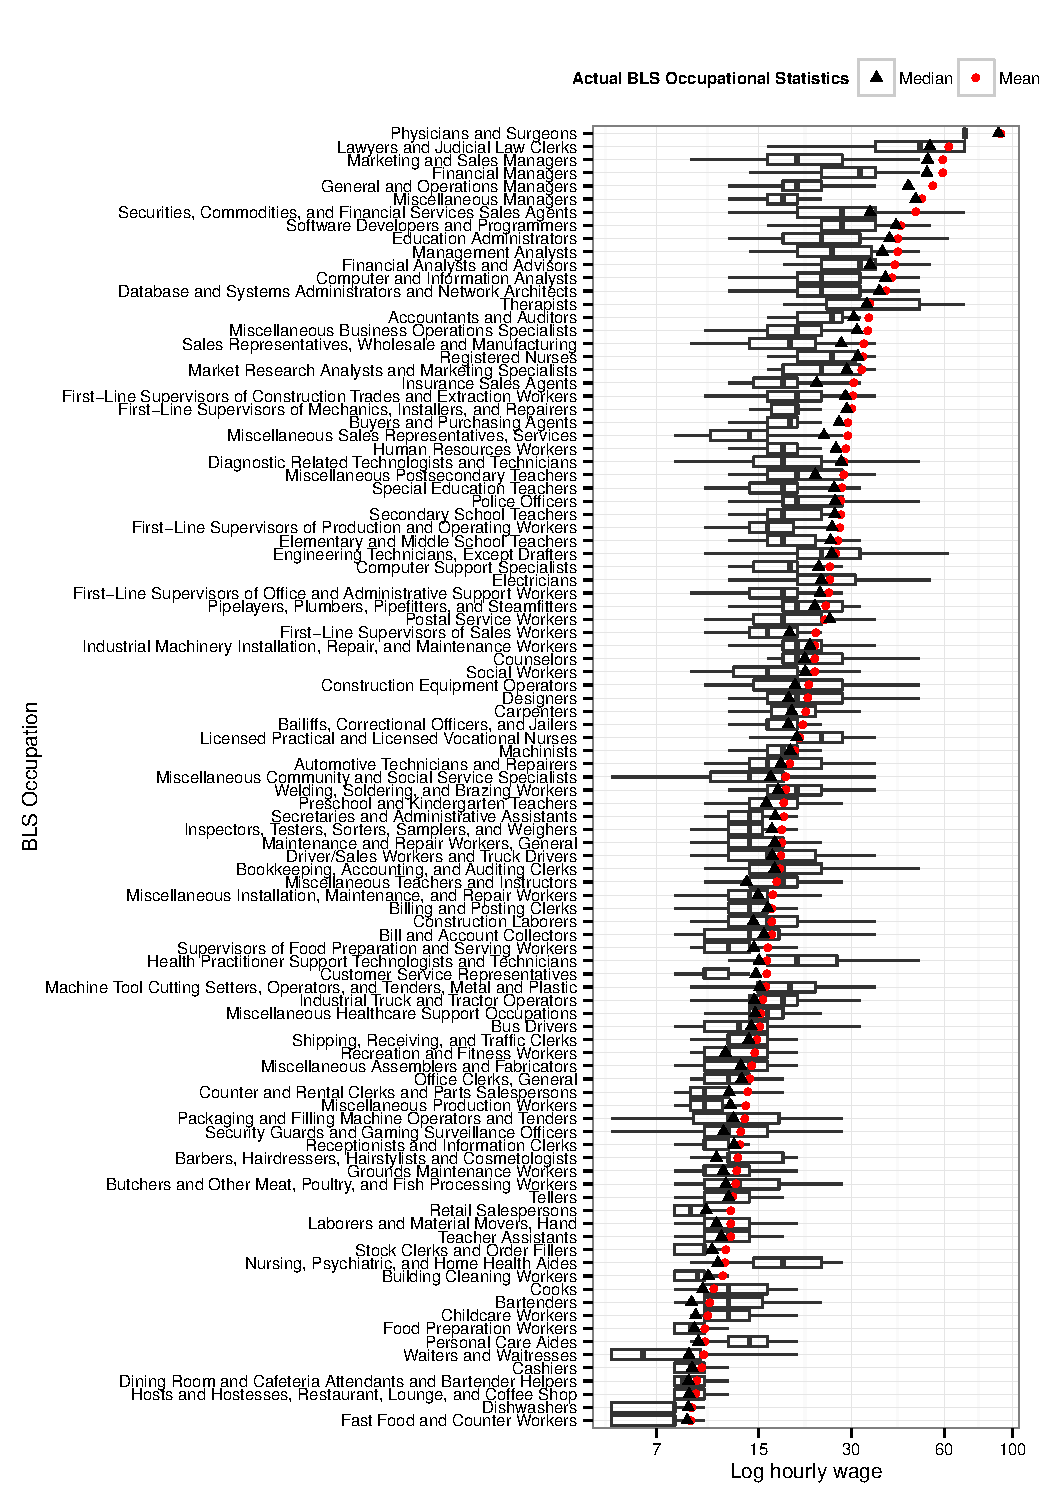
\includegraphics[width = \linewidth]{./plots/box_plots_by_occupation.pdf} 
\end{figure} 

Figure~\ref{fig:prediction_scatter} shows the scatter plot of predicted wages verus actual hourly wages. 

\begin{figure}
\caption{Perceived hourly wages versus actual hourly wages \label{fig:prediction_scatter}} 
\centering 
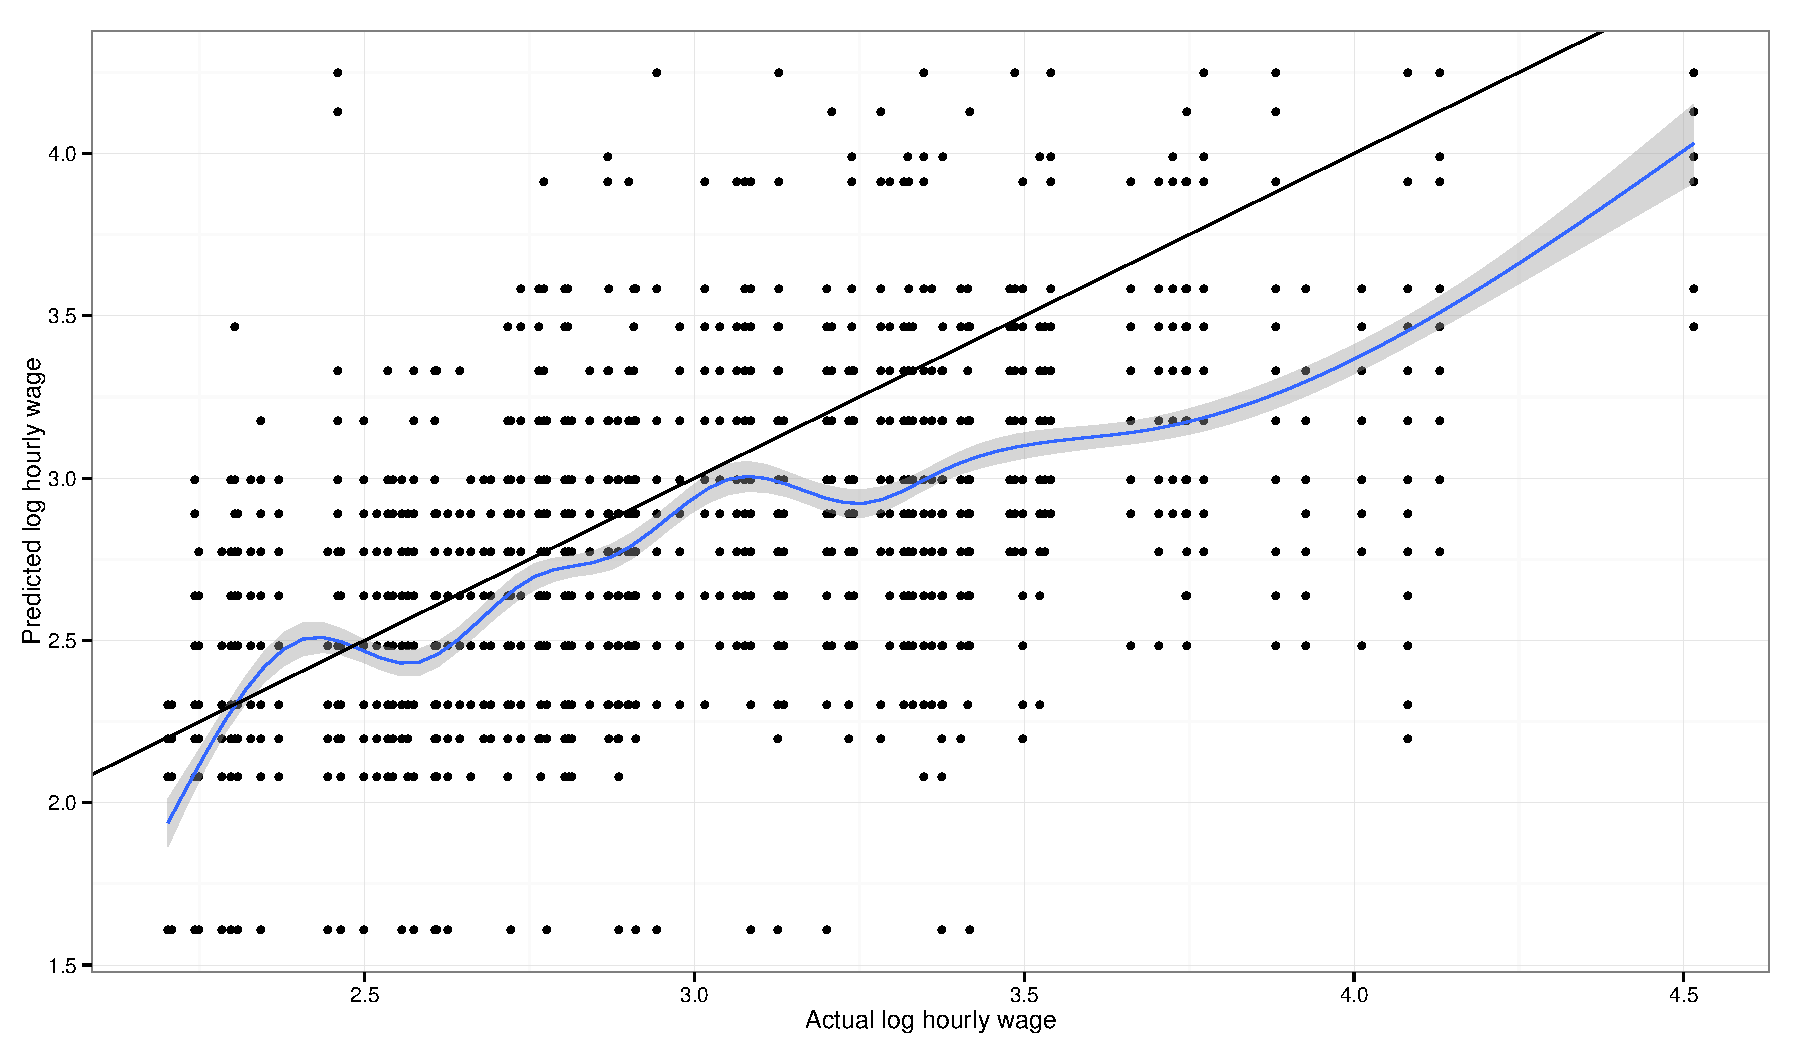
\includegraphics[width = \linewidth]{./plots/prediction_scatter.pdf} 
\end{figure} 

\subsection{Clustering} 

\begin{table}
\centering 
\caption{Clustering of social knowledge by wage}
%%%%%%%%%%%%%%%%%%%%%%%%%%%%%%%%%%%%%%%%%%%%%%%%%%%%%%%%%%%%%%%%%%%%%%%%%%%%%%%%%%%%%%%%%%%%%%%%%%%%%%%%%%%%%%%%%%%%%%%%%%%%%%%%%%%%%%%%%%%%%%
%
% Calls:
% (1):  lm(formula = I(social > -2) ~ log(actual.mean.wage) * mean.wage.others.social + log(tot.emp), data = by.worker.df) 
% (2):  lmer(formula = I(social > -2) ~ log(actual.mean.wage) * mean.wage.others.social + log(tot.emp) + (1 | WorkerId), data = by.worker.df) 
% (3):  lmer(formula = I(social > -2) ~ log(actual.mean.wage) * mean.wage.others.social + (1 | WorkerId) + (1 | title), data = by.worker.df) 
%
%%%%%%%%%%%%%%%%%%%%%%%%%%%%%%%%%%%%%%%%%%%%%%%%%%%%%%%%%%%%%%%%%%%%%%%%%%%%%%%%%%%%%%%%%%%%%%%%%%%%%%%%%%%%%%%%%%%%%%%%%%%%%%%%%%%%%%%%%%%%%%
\begin{tabular}{lcD{.}{.}{7}cD{.}{.}{7}cD{.}{.}{7}}
\toprule
&&\multicolumn{1}{c}{(1)} && \multicolumn{1}{c}{(2)} && \multicolumn{1}{c}{(3)}\\
\midrule
(Intercept)                                             &  &  3.574^{***} &&  2.699^{**}  &&  4.880^{***}\\
                                                        &  &  (1.015)     &&  (0.977)     &&  (0.929)    \\
log(actual.mean.wage)                                   &  & -1.510^{***} && -1.244^{***} && -1.390^{***}\\
                                                        &  &  (0.327)     &&  (0.306)     &&  (0.296)    \\
mean.wage.others.social                                 &  & -1.626^{***} && -1.318^{***} && -1.406^{***}\\
                                                        &  &  (0.332)     &&  (0.320)     &&  (0.307)    \\
log(tot.emp)                                            &  &  0.131^{***} &&  0.131^{***} &&             \\
                                                        &  &  (0.015)     &&  (0.014)     &&             \\
log(actual.mean.wage) $\times$ mean.wage.others.social &  &  0.504^{***} &&  0.415^{***} &&  0.447^{***}\\
                                                        &  &  (0.109)     &&  (0.102)     &&  (0.098)    \\
Var((Intercept)|WorkerId)                               &  &              &&   0.045      &&   0.040     \\
                                                        &  &              &&              &&             \\
Var(|Residual)                                          &  &              &&   0.198      &&   0.179     \\
                                                        &  &              &&              &&             \\
Var((Intercept)|title)                                  &  &              &&              &&   0.027     \\
                                                        &  &              &&              &&             \\
\midrule
R-squared                                               &  &      0.040   &&              &&             \\
adj. R-squared                                          &  &      0.039   &&              &&             \\
sigma                                                   &  &      0.489   &&              &&             \\
F                                                       &  &     26.252   &&              &&             \\
p                                                       &  &      0.000   &&              &&             \\
Log-likelihood                                          &  &  -1754.623   &&  -1609.371   &&  -1555.602  \\
Deviance                                                &  &    596.067   &&   3218.743   &&   3111.204  \\
AIC                                                     &  &   3521.245   &&   3232.743   &&   3125.204  \\
BIC                                                     &  &   3556.182   &&   3273.503   &&   3165.964  \\
N                                                       &  &   2497       &&   2497       &&   2497      \\
\bottomrule
\end{tabular}
 
\end{table} 


\begin{figure}
\caption{Wage trends} 
\centering
\begin{minipage}{0.85 \linewidth}
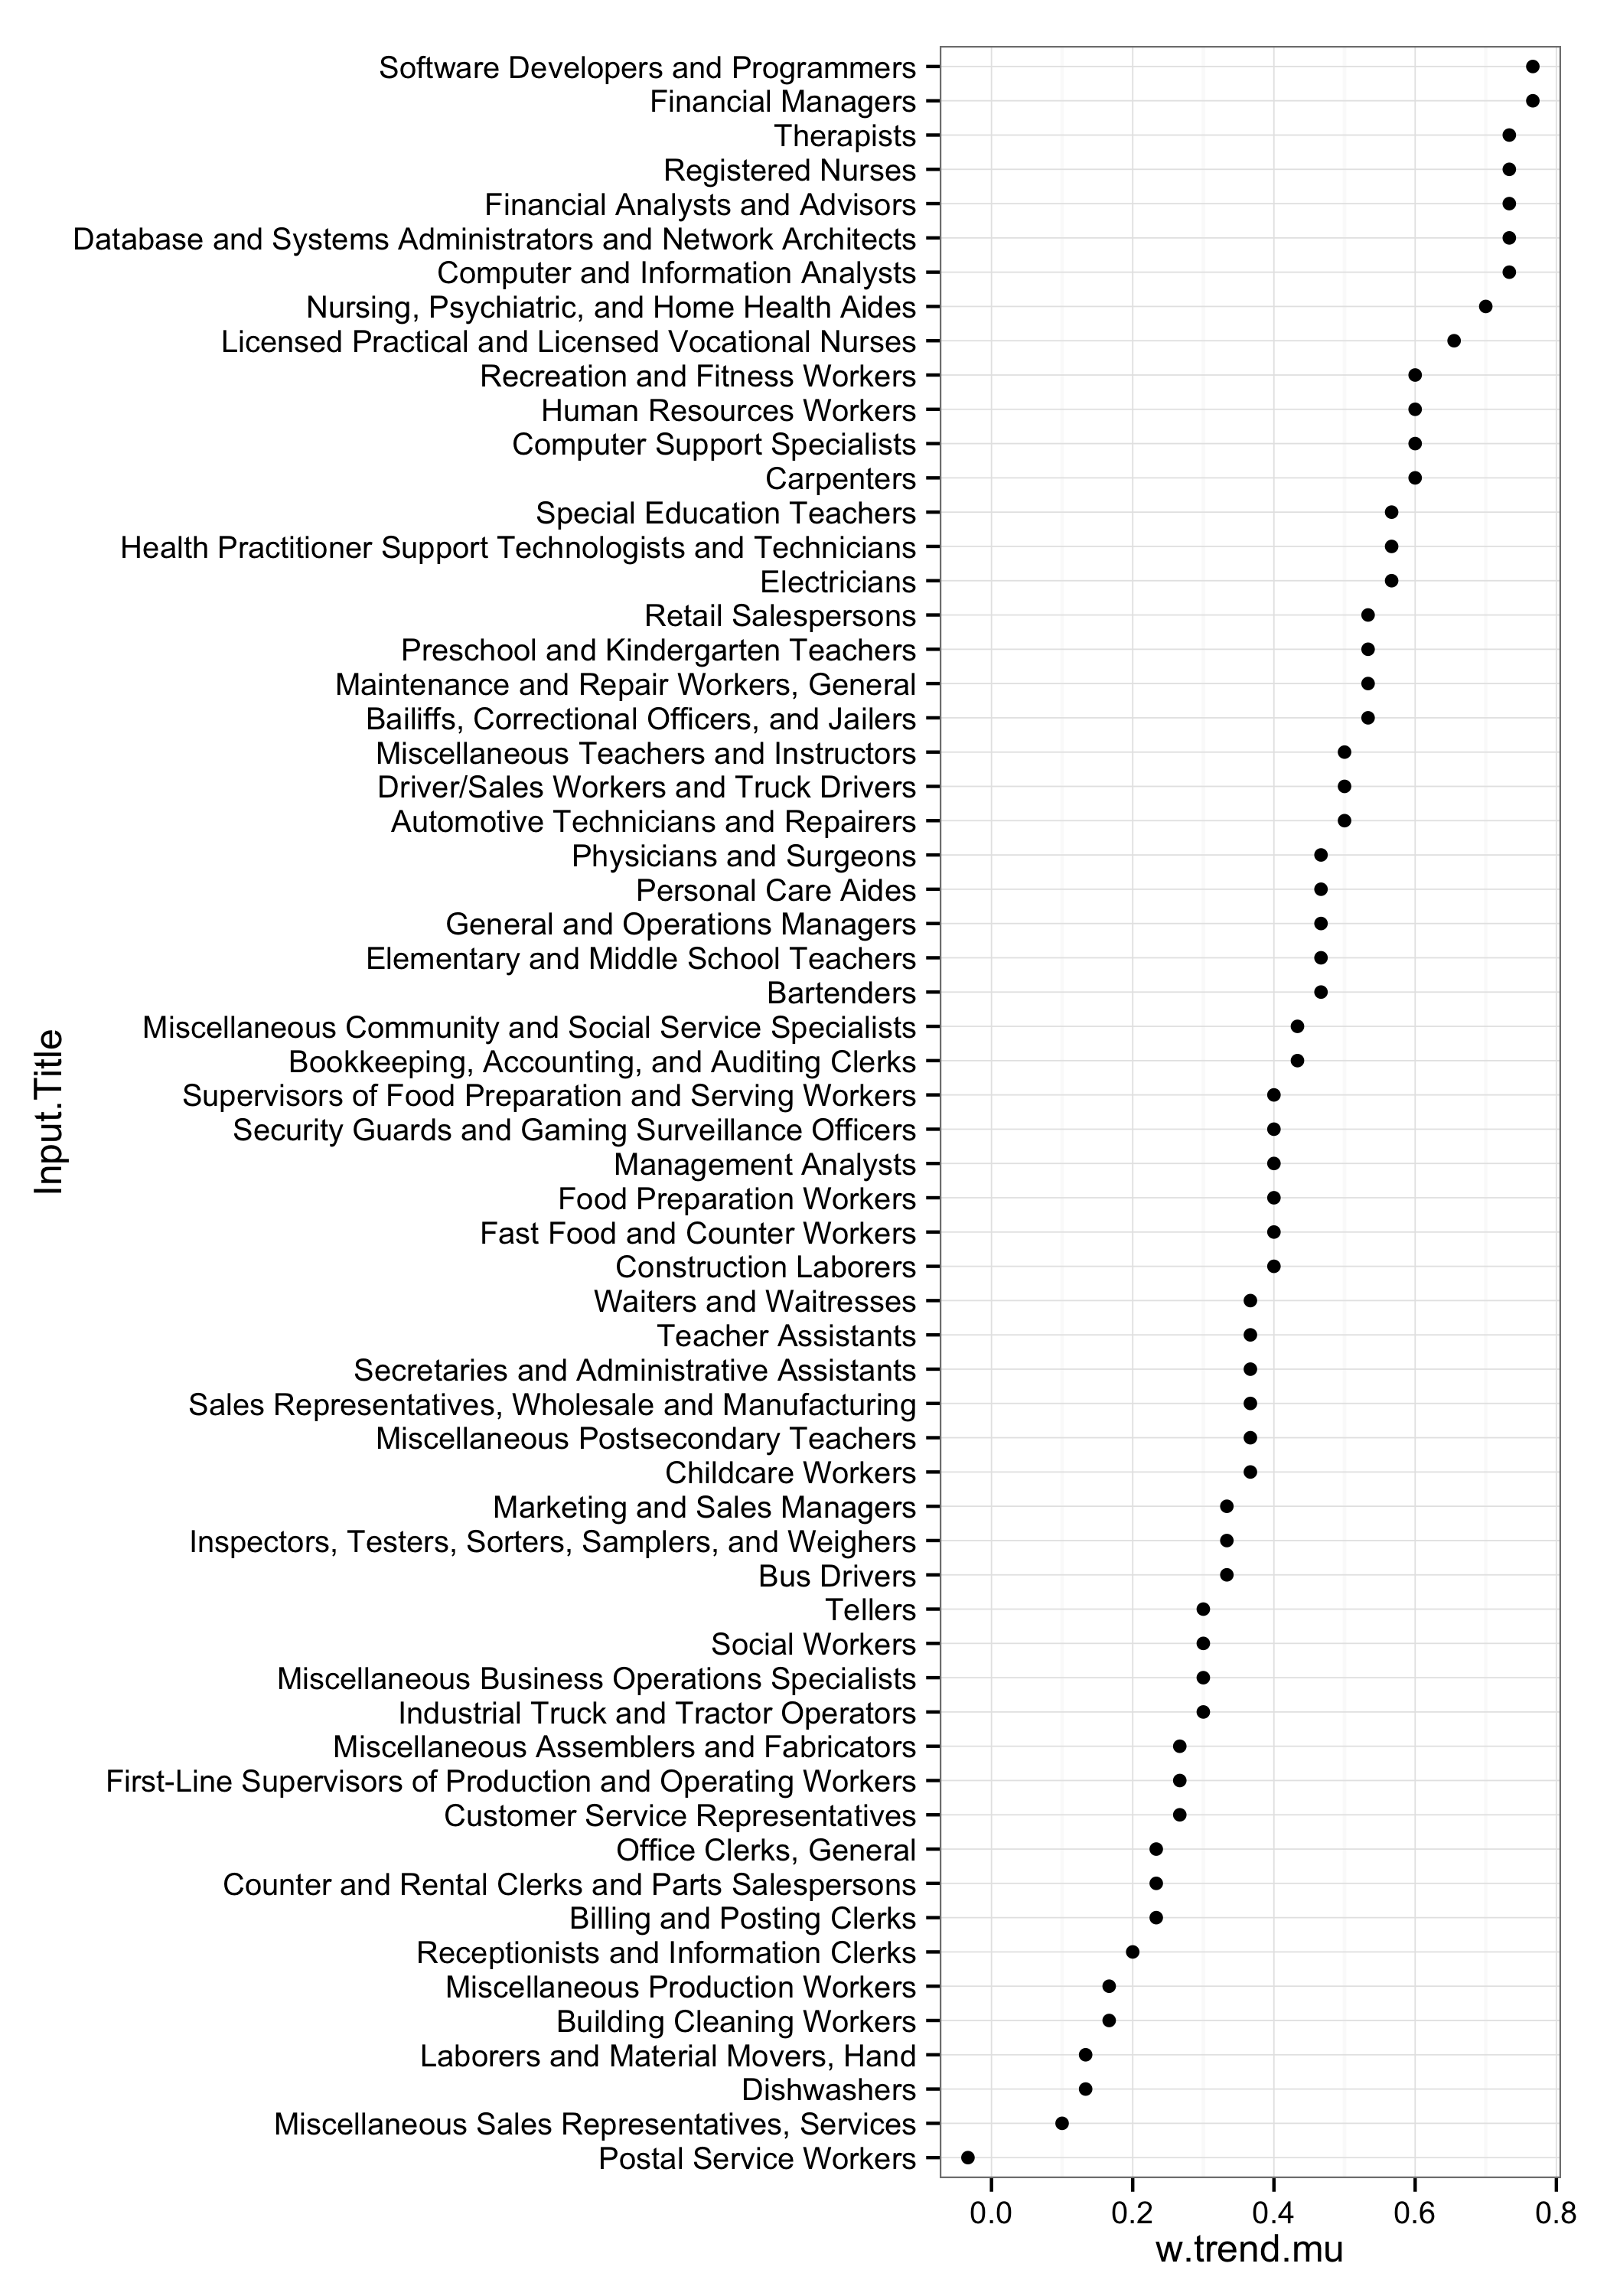
\includegraphics[width = \linewidth]{./plots/wage_trends.png}
\end{minipage}  
\end{figure} 


\begin{figure}
\caption{Knowledge by total employment} 
\centering
\begin{minipage}{0.85 \linewidth}
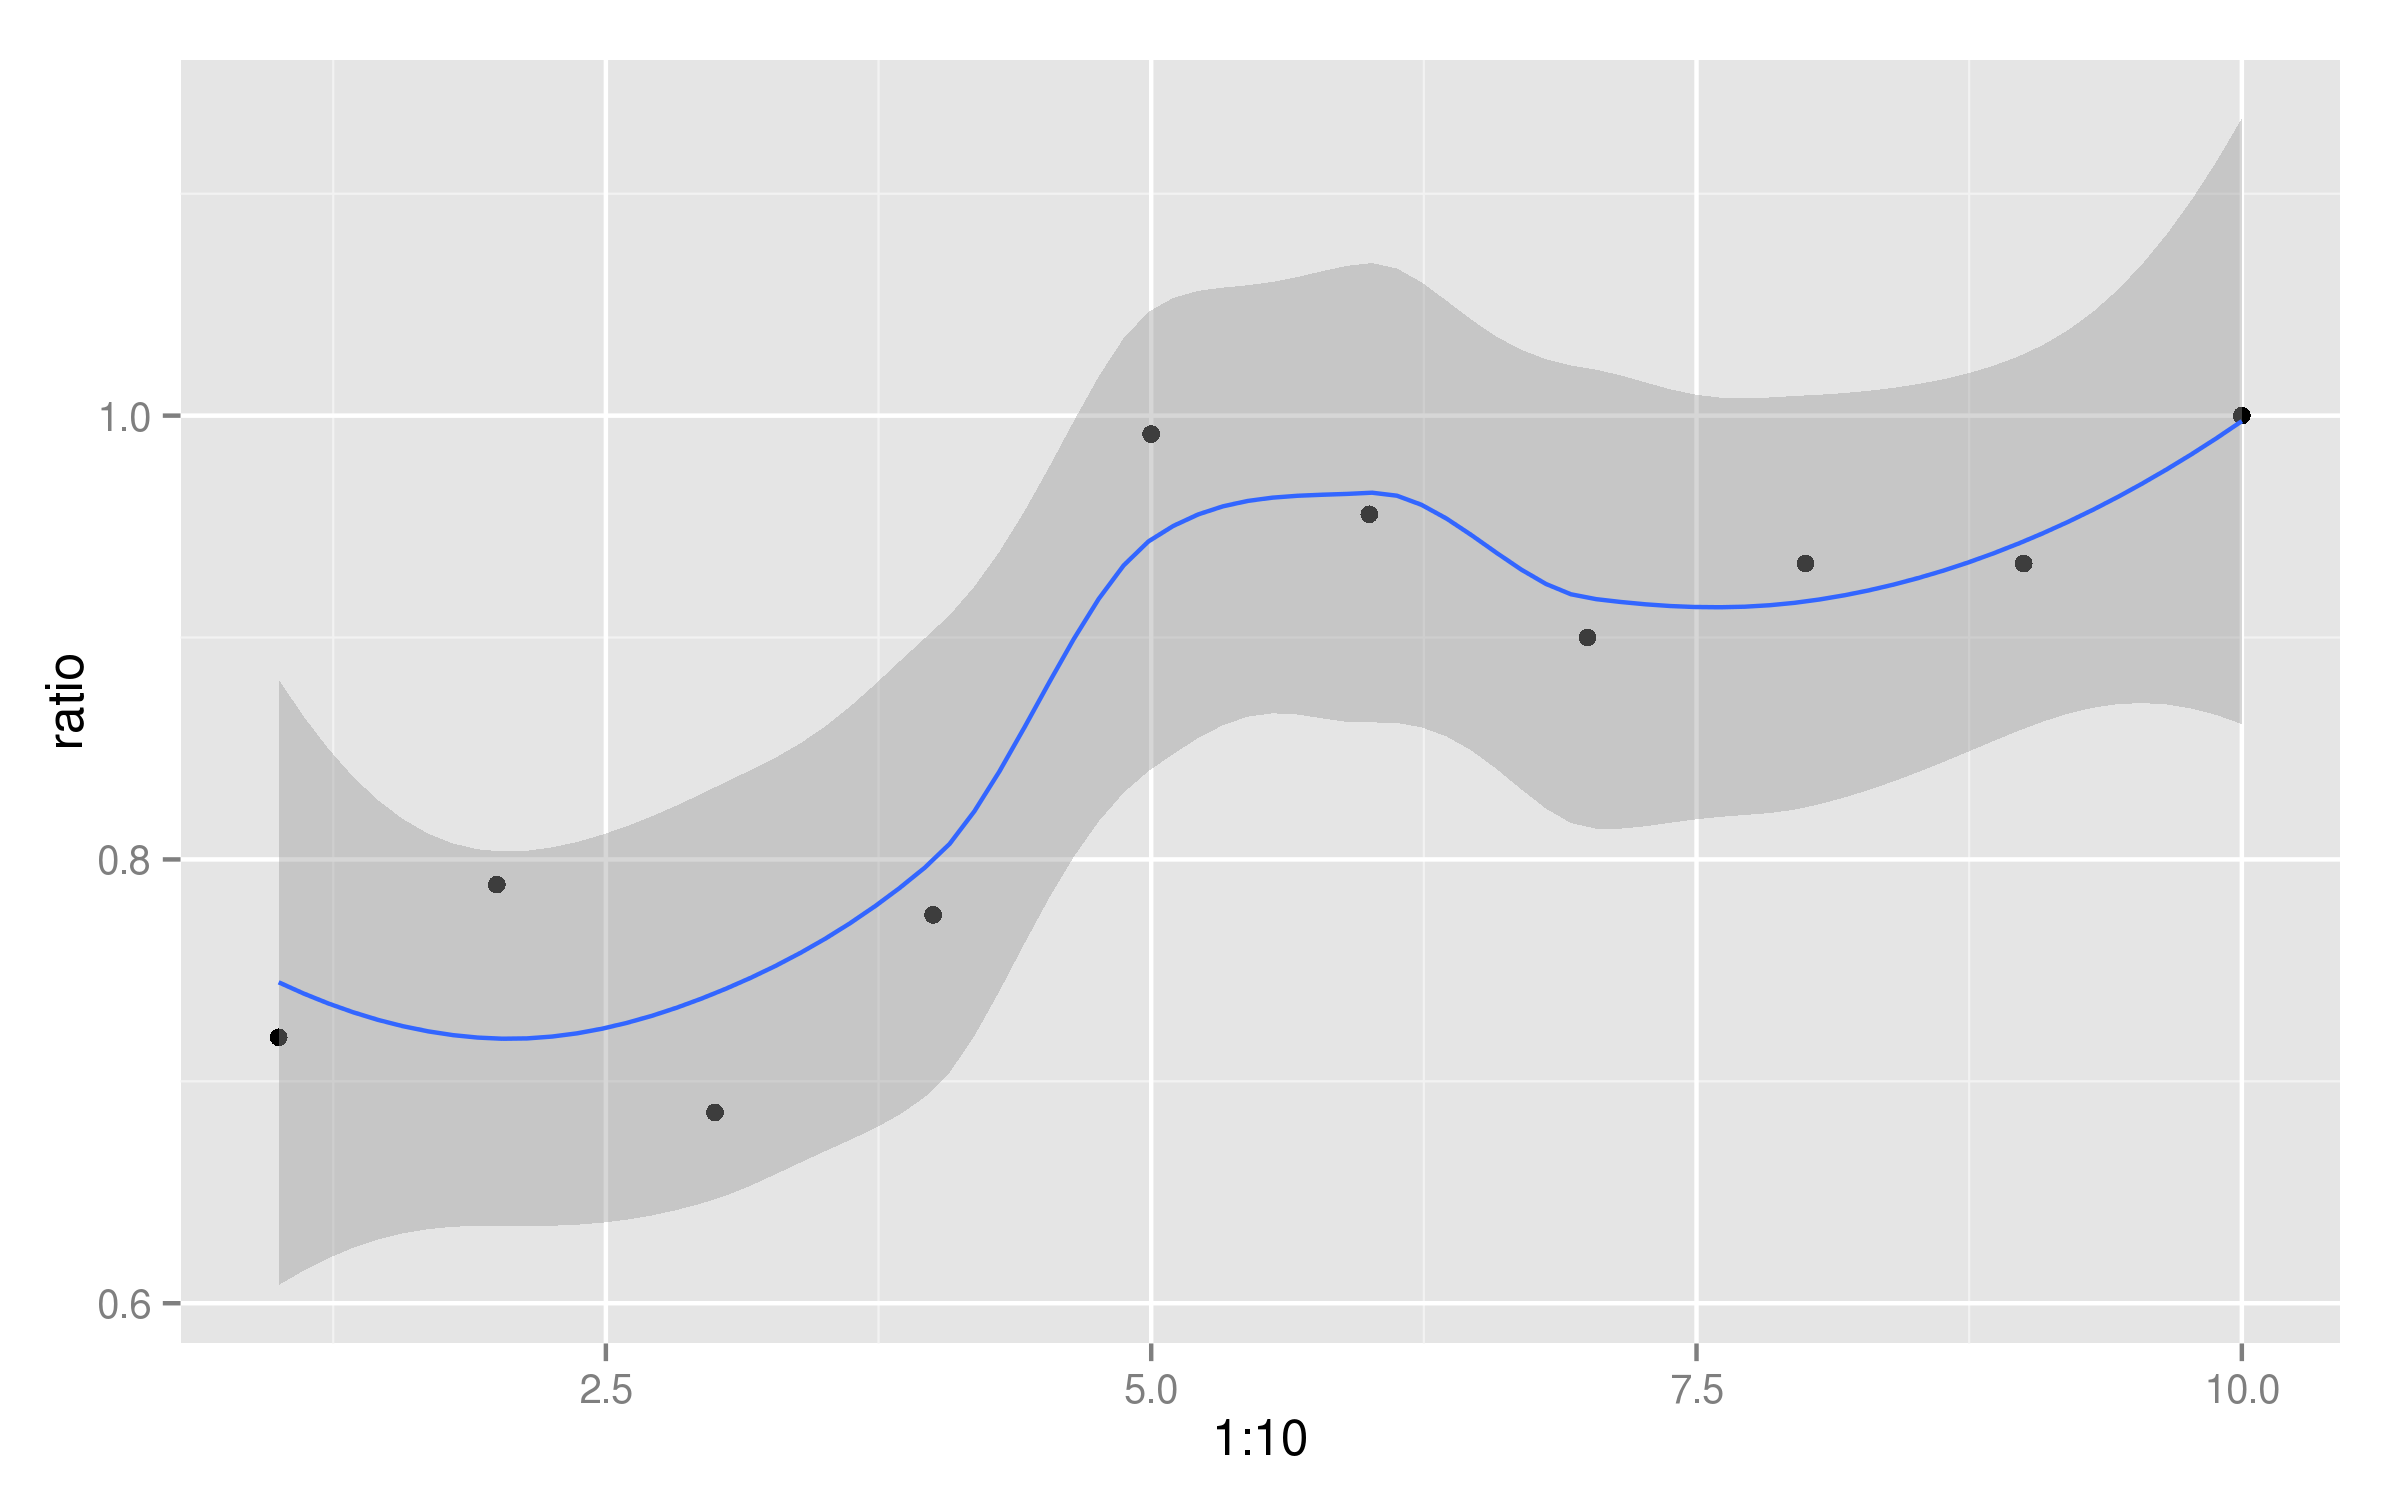
\includegraphics[width = \linewidth]{./plots/knowledge_emp.png}
\end{minipage}  
\end{figure} 




%% latex table generated in R 3.0.2 by xtable 1.7-1 package
% Tue Nov 12 04:22:34 2013
\begin{table}[ht]
\centering
\begin{tabular}{rll}
  \hline
 &      OES &      MTSO \\ 
  \hline
1 & Min.   :0.0000   & Min.   :18.05   \\ 
  2 & 1st Qu.:0.5000   & 1st Qu.:28.54   \\ 
  3 & Median :0.7000   & Median :32.14   \\ 
  4 & Mean   :0.7152   & Mean   :34.29   \\ 
  5 & 3rd Qu.:0.9000   & 3rd Qu.:39.77   \\ 
  6 & Max.   :1.4000   & Max.   :60.57   \\ 
   \hline
\end{tabular}
\caption{RSE for Hourly Wages in OES and MTSO datasets (all obs.)} 
\label{tab:rse_oes_mtso1}
\end{table}

%% latex table generated in R 3.0.2 by xtable 1.7-1 package
% Tue Nov 12 04:22:47 2013
\begin{table}[ht]
\centering
\begin{tabular}{rll}
  \hline
 &      OES &      MTSO \\ 
  \hline
1 & Min.   :0.0000   & Min.   :15.01   \\ 
  2 & 1st Qu.:0.5000   & 1st Qu.:25.82   \\ 
  3 & Median :0.7000   & Median :30.96   \\ 
  4 & Mean   :0.7173   & Mean   :32.69   \\ 
  5 & 3rd Qu.:0.9000   & 3rd Qu.:40.00   \\ 
  6 & Max.   :1.4000   & Max.   :65.93   \\ 
  7 &  & NA's   :2   \\ 
   \hline
\end{tabular}
\caption{RSE for Hourly Wages in OES and MTSO datasets (filtered)} 
\label{tab:rse_oes_mtso2}
\end{table}


\begin{small} 
%%%%%%%%%%%%%%%%%%%%%%%%%%%%%%%%%%%%%%%%%%%%%%%%%%%%%%%%%%%%%%%%%%%%%%%%%%%%%%%%%%%%%%%%%%%%%%%%%%%%%%%%%%%%%%%%%%%%%%%%%%%%%
%
% Calls:
% 1:  glm(formula = error ~ know * social + log(TOT_EMP) + H_WAGE, data = mturk.df) 
% 2:  glm(formula = error ~ know * social + H_WAGE, data = mturk.df) 
% 3:  glm(formula = error ~ social + H_WAGE + log(TOT_EMP), data = mturk.df) 
% 4:  lmer(formula = error ~ know * social + log(TOT_EMP) + H_WAGE + (1 | Input.Title), data = mturk.df) 
% 5:  glm(formula = error ~ know * social + log(TOT_EMP) + H_WAGE + I(log(Answer.wage) > 3), data = mturk.df) 
%
%%%%%%%%%%%%%%%%%%%%%%%%%%%%%%%%%%%%%%%%%%%%%%%%%%%%%%%%%%%%%%%%%%%%%%%%%%%%%%%%%%%%%%%%%%%%%%%%%%%%%%%%%%%%%%%%%%%%%%%%%%%%%
\begin{tabular}{lcD{.}{.}{7}cD{.}{.}{7}cD{.}{.}{7}cD{.}{.}{7}cD{.}{.}{7}}
\toprule
&&\multicolumn{1}{c}{1} && \multicolumn{1}{c}{2} && \multicolumn{1}{c}{3} && \multicolumn{1}{c}{4} && \multicolumn{1}{c}{5}\\
\midrule
(Intercept)                  &  &  -0.058      &&  0.137^{***} &&   0.004      &&  -0.025      &&   0.034     \\
                             &  &  (0.121)     &&  (0.038)     &&  (0.117)     &&  (0.274)     &&  (0.116)    \\
know                         &  &   0.043      &&   0.046      &&              &&   0.035      &&   0.048     \\
                             &  &  (0.038)     &&  (0.038)     &&              &&  (0.035)     &&  (0.036)    \\
social                       &  & -0.042^{*}   && -0.041^{*}   && -0.013^{*}   &&  -0.033      && -0.037^{*}  \\
                             &  &  (0.019)     &&  (0.019)     &&  (0.006)     &&  (0.018)     &&  (0.018)    \\
log(TOT_EMP)                 &  &   0.014      &&              &&   0.013      &&   0.012      &&   0.007     \\
                             &  &  (0.008)     &&              &&  (0.008)     &&  (0.020)     &&  (0.008)    \\
H_WAGE                       &  &  0.008^{***} &&  0.007^{***} &&  0.008^{***} &&  0.008^{***} &&  0.010^{***}\\
                             &  &  (0.000)     &&  (0.000)     &&  (0.000)     &&  (0.001)     &&  (0.000)    \\
know $\times$ social        &  &   0.036      &&   0.037      &&              &&   0.025      &&  0.037^{*}  \\
                             &  &  (0.020)     &&  (0.020)     &&              &&  (0.018)     &&  (0.019)    \\
Var((Intercept)|Input.Title) &  &              &&              &&              &&   0.014      &&             \\
                             &  &              &&              &&              &&              &&             \\
Var(|Residual)               &  &              &&              &&              &&   0.062      &&             \\
                             &  &              &&              &&              &&              &&             \\
I(log(Answer.wage) > 3)      &  &              &&              &&              &&              && -0.198^{***}\\
                             &  &              &&              &&              &&              &&  (0.013)    \\
\midrule
Aldrich-Nelson R-sq.         &  &      0.011   &&      0.011   &&      0.011   &&              &&      0.017  \\
McFadden R-sq.               &  &      0.133   &&      0.132   &&      0.129   &&              &&      0.201  \\
Cox-Snell R-sq.              &  &      0.011   &&      0.011   &&      0.011   &&              &&      0.017  \\
Nagelkerke R-sq.             &  &      0.138   &&      0.137   &&      0.134   &&              &&      0.208  \\
phi                          &  &      0.075   &&      0.075   &&      0.075   &&              &&      0.069  \\
Likelihood-ratio             &  &     30.588   &&     30.374   &&     29.807   &&              &&     46.063  \\
p                            &  &      0.000   &&      0.000   &&      0.000   &&              &&      0.000  \\
Log-likelihood               &  &   -326.545   &&   -327.977   &&   -333.184   &&   -184.475   &&   -218.938  \\
Deviance                     &  &    199.028   &&    199.242   &&    200.475   &&    368.950   &&    183.553  \\
AIC                          &  &    667.091   &&    667.955   &&    676.367   &&    384.950   &&    453.877  \\
BIC                          &  &    708.291   &&    703.269   &&    705.811   &&    432.036   &&    500.962  \\
N                            &  &   2659       &&   2659       &&   2667       &&   2659       &&   2659      \\
\bottomrule
\end{tabular}
 
\end{small} 

\begin{tiny} 
\caption{Know anyone}


\usepackage{booktabs}
\begin{table}
\begin{center}
\begin{tabular}{l c c c }
\toprule
               & Model 1 & Model 2 & Model 3 \\
\midrule
(Intercept)    & $-0.50^{***}$ & $0.42$      & $-0.57^{*}$  \\
               & $(0.06)$      & $(0.22)$    & $(0.25)$     \\
TOT_EMP        & $0.00^{***}$  &             & $0.00^{***}$ \\
               & $(0.00)$      &             & $(0.00)$     \\
log(H_WAGE)    &               & $-0.18^{*}$ & $0.02$       \\
               &               & $(0.07)$    & $(0.08)$     \\
\midrule
AIC            & 4029.23       & 4104.78     & 4031.16      \\
BIC            & 4041.23       & 4116.78     & 4049.15      \\
Log Likelihood & -2012.62      & -2050.39    & -2012.58     \\
Deviance       & 4025.23       & 4100.78     & 4025.16      \\
Num. obs.      & 2969          & 2969        & 2969         \\
\bottomrule
\multicolumn{4}{l}{\scriptsize{\textsuperscript{***}$p<0.001$, 
  \textsuperscript{**}$p<0.01$, 
  \textsuperscript{*}$p<0.05$}}
\end{tabular}
\caption{Statistical models}
\label{table:coefficients}
\end{center}
\end{table}

 
\end{tiny} 

\bibliographystyle{plain}
\bibliography{kwow.bib}

\end{document} 
